\documentclass[12pt, a4paper]{article}
\usepackage{authblk}
\usepackage{graphicx}
\usepackage{placeins}
\usepackage{ragged2e}

\begin{document}
\title{Uni Variant Data Analysis Project}
\author{\textbf {Bushra Naeemi}}
\affil[] {The American University of Afghanistan

Division of Science, Technology, and Mathematics

Instructor: Asadullah Jawid}
\date{\today}
\maketitle
\newpage
\tableofcontents
\newpage
\section{Summary}
The data is about the farmers from 3 provinces. farmers has been asked about their personal informations like age and gender, and their family members. Also about the income, accupation, crop net income, and rainfall.  
\section{Introduction}
\justify
The data set is from 3 provinces and. It has been taken from the farmers about their farms. We have both numeric and categorical data, each has been categorized in columns.


\subsection{Numerical Variable}
\textbf{Work.on.farm.FAMILY:} Shows the number of family members working in the farm \\
\textbf{Work.off.farm.Family:} Shows the number of family members not working in the farm.\\
\textbf{X.Not..employed...:} number of net employed.\\
\textbf{Female..work.on.farm:} Number of Female working in farm.\\
\textbf{Crop.Net.Income:} Crop net income of farmer.\\
\textbf{t4:} Shows the temperature in the specific area in April.\\
\textbf{r4:} Shows the rainfall in the specific area in April.\\
\subsection{Sample}
Data has been collected from three provinces. 
\section{Methods}
 To analyze data we used a combination of both numerical measures and graphical methods. more   specifically:\\\\
 \textbf{Numerical Measures:}\\
 - Mean( Measures of Central tendency)\\
 - Standard Deviation and Range( Dispersion)\\
 - skewness and kurtosis(Distribution)\\\\
 \textbf{Graphical Methods:}\\
- Piechart(categorical variables)\\
-  Density plot(numerical variables)\\
-  histogram(numerical variables)\\
-  boxplot(numerical varibale.

\section{Results and Discussions}
\subsection{Numerical Variable}
\textbf{Statistics of Numerical Variables:}
%latex.default(Table, "table1.tex")%
\begin{table}[h]

\begin{center}
\begin{tabular}{ccccccc}
\hline\hline
\multicolumn{1}{c}{Variable}&\multicolumn{1}{c}{Mean}&\multicolumn{1}{c}{Std.Dev}&\multicolumn{1}{c}{Minimum}&\multicolumn{1}{c}{Maximum}&\multicolumn{1}{c}{Skewness}&\multicolumn{1}{c}{Kurtosis}\tabularnewline
\hline

$X.Not..employed...$&$  5.286$&$ 6.188$&$ -191.0$&$  33.0$&$-21.09$&$671.57$\tabularnewline
$Female..work.on.farm$&$1.718$&$ 1.353$&$ 0.000$&$ 10.00$&$1.286$&$3.452$\tabularnewline
$Crop.Net.Income$&$78369.5$&$ 287632.5$&$ -951500$&$7089500$&$ 14.147$&$279.70$\tabularnewline
$t4$&$4.726$&$2.997$&$ 0.217$&$ 11.514$&$0.2628$&$-1.1044$\tabularnewline
$r4$&$60.021$&$27.843$&$ 28.932$&$123.623$&$0.853$&$-0.682$\tabularnewline
\hline
\end{tabular}\end{center}
\caption{Descriptive Statistics of Numerical Variables}
\end{table}
\justify
\textbf{numeric values from table}\\  
Tabel 1 The table above shows the comparison between the numeric values based of mean, standard deviation, minimum maximum, skewness, and kurtosis.


\begin{figure}[h]
\centering
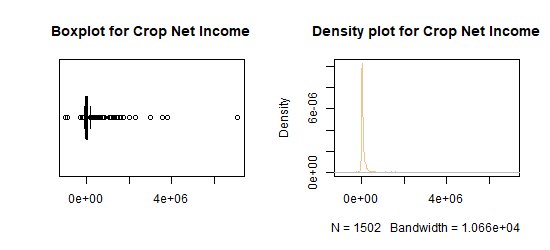
\includegraphics[scale=.5]{income.png}
\caption{The box plot of Crop net income with the outliers with causes problems}
\end{figure}
\begin{figure}[h]
\centering
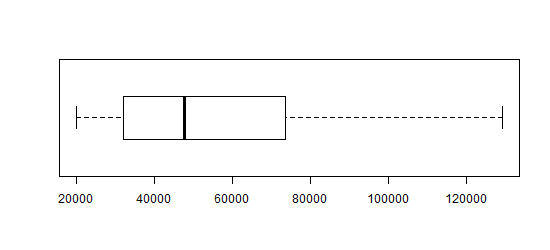
\includegraphics[scale=.5]{income2.png}
\caption{The box plot of Crop net income without outliers}
\end{figure}
\begin{figure}[h]
\centering
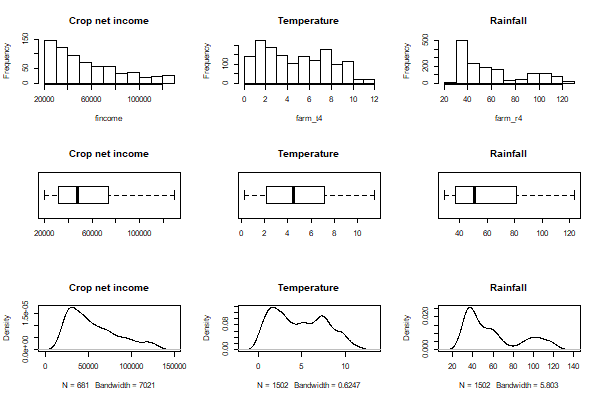
\includegraphics[scale=.5]{variables.png}
\caption{The comparison between Income rainfall and temperature by graphs}
\end{figure}


\subsection{Categorical Variable}
\textbf{Importance.of.farming.0.not.atll.Impornt.1.importnt.2.Very.impornt}: Shows the importance of farming for the farmers.\\
\begin{table}[h!]
\begin{center}
\caption{Summary Statistics of Categorical Variables}
\begin{tabular}{llrl}
\hline
Variable & Categories & Counts & Percent\\
\hline
\hline
Importance.of.farming.0.not.atll.Impornt.1.importnt.2.Very.impornt& not.atall[0]important[1]Very.important[2]& [199][364][939] & [13][24][63]\\

\end{tabular}
\end{center}
\end{table}

\begin{figure}[h]
\centering
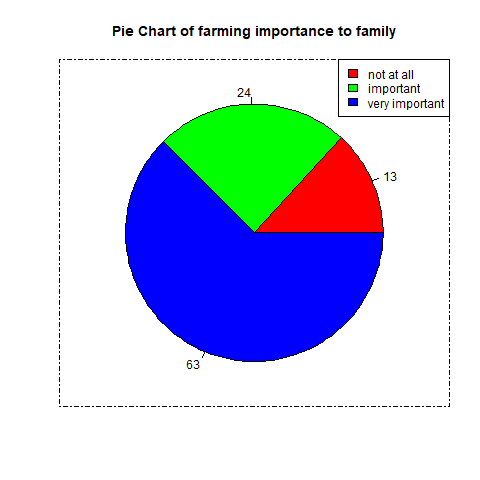
\includegraphics[scale=.5]{farmimportance.png}
\caption{The pie chart of importance of farming for farmers}
\end{figure}
\textbf{importance of farming}\\  
The pie chart shows that 13 percent of farmers think that farming is not important at all, 24 percent think that farming is important, and 63 percent of farmers think that farming is very important.

\subsection{Sub-Sample Analysis}
\textbf{Crop Net Income, Temperature, Rainfall in 3 provinces}\\  
In this section we show the Crop Net Income in province 1, province 2, and province 3.
The temperature in province 1, province 2, and province 3.
The rainfall in province 1, province 2, and province 3.
\begin{figure}[h]
\centering
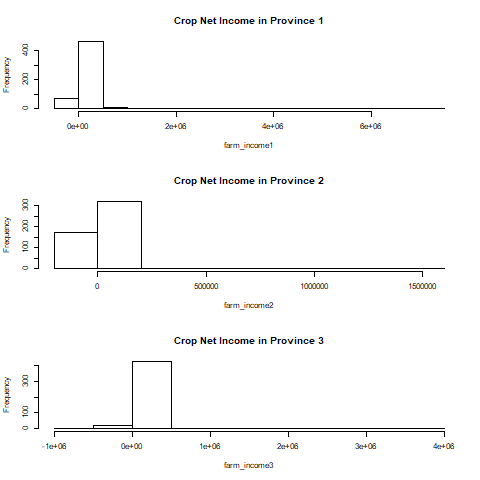
\includegraphics[scale=.5]{cropnetin.png}
\caption{The Net income of 3 provinces}
\end{figure}
\begin{figure}[h]
\centering
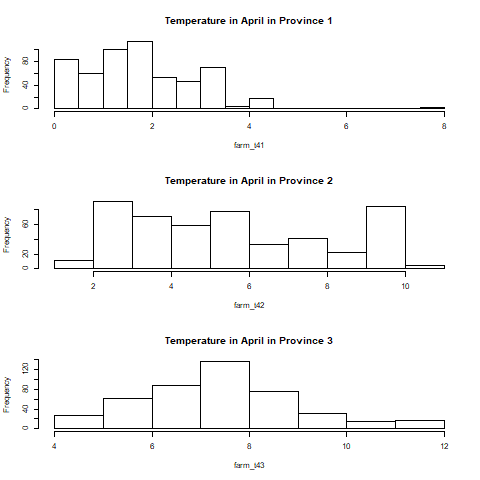
\includegraphics[scale=.5]{tem4.png}
\caption{The temperature of 3 provinces}
\end{figure}
\begin{figure}[h]
\centering
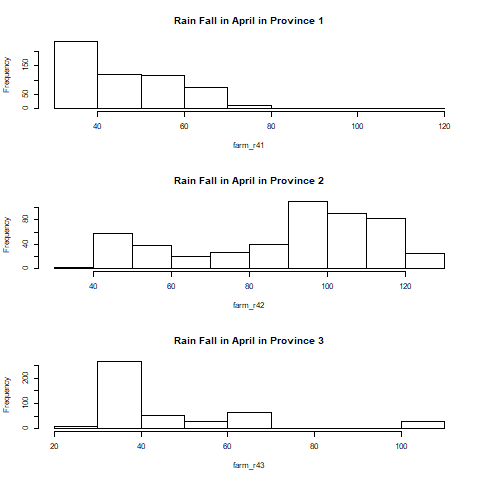
\includegraphics[scale=.5]{rain4.png}
\caption{The rainfall of 3 provinces}
\end{figure}
\end{document}
